

%-------------------------------------------------------------------------------
% Dokumenten Klasse
\documentclass[
	final,
	a4paper,
	oneside,
	parskip=full,
	headings=standardclasses,
	headings=big,
	pointednumbers
]{scrartcl}

%-------------------------------------------------------------------------------
% Packete nutzen
\usepackage{ngerman,palatino,setspace}
\usepackage[T1]{fontenc}
\usepackage[utf8]{inputenc}
\usepackage[left=20mm,right=20mm,top=25mm,bottom=25mm]{geometry}
\usepackage{amsmath}
\usepackage{mathtools}
\usepackage{tikz}

\usetikzlibrary{automata, positioning, arrows}

%{
%\tikzset{
%    ->, % makes the edges directed
%    >=stealth, % makes the arrow heads bold
%    node distance=2cm, % specifies the minimum distance between two nodes. Change if necessary.
%    every state/.style={thick, fill=gray!10}, % sets the properties for each ’state’ node
%    every edge/.append style={line width=0.25mm}, % sets the properties for each ’state’ node
%    initial text=$ $, % sets the text that appears on the start arrow
%}
%}

\tikzset{
    node distance=2cm, % Minimum distance between two nodes. Change if necessary.
    every state/.style={ % Sets the properties for each state
        semithick,
        fill=gray!10
    },
    initial text={}, % No label on start arrow
    double distance=2pt, % Adjust appearance of accept states
    every edge/.style={ % Sets the properties for each transition
        draw,
        ->,>=stealth, % Makes edges directed with bold arrowheads
        auto,
        semithick
    },
    shift left/.style ={commutative diagrams/shift left={#1}},
    shift right/.style={commutative diagrams/shift right={#1}}
}

%-------------------------------------------------------------------------------
\usepackage{multirow}

%-------------------------------------------------------------------------------
% mdframed
\usepackage[framemethod=tikz]{mdframed}

\mdfsetup{%
    leftmargin=0cm,
    skipabove=0.2cm,
    linecolor=black,
    backgroundcolor=gray!10,
    linewidth=0.50pt,
    innerleftmargin=0.2cm,
    innerrightmargin=0.0cm,
    innertopmargin=-0.2cm,
    innerbottommargin=0.1cm
}

\newmdenv[
    font=\small,
    innerleftmargin=0.2cm,
    innerrightmargin=0.0cm,
    innertopmargin=-0.2cm,
    innerbottommargin=0.1cm
]{mdmath}


%-------------------------------------------------------------------------------
% uline
\usepackage{ulem}

%-------------------------------------------------------------------------------
% mycircle
\newcommand{\mycircle}[1]{%
    \tikz[baseline=(char.base)]\node[rectangle, rounded corners, draw=red, inner sep=2pt](char){#1} ;}

%-------------------------------------------------------------------------------
% Dokument
\begin{document}
    
    
    %--- Page 1 --------------------------------------------------------------------
    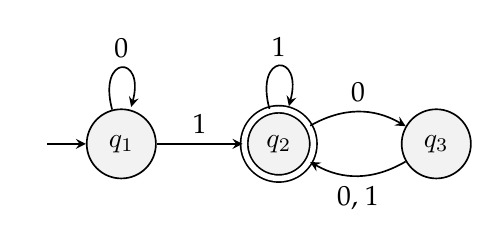
\begin{tikzpicture}
        \node[state, initial] (q1) {$q_1$};
        \node[state, accepting, right of=q1] (q2) {$q_2$};
        \node[state, right of=q2] (q3) {$q_3$};
        \draw (q1) edge[loop above] node{0} (q1)
        (q1) edge[above] node{1} (q2)
        (q2) edge[loop above] node{1} (q2)
        (q2) edge[bend left, above] node{0} (q3)
        (q3) edge[bend left, below] node{0, 1} (q2);
    \end{tikzpicture}

    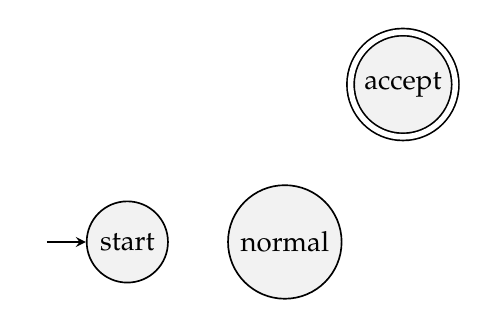
\begin{tikzpicture}
        \node[state] at (0, 0) (q1) {normal};
        \node[state, initial, left of=q1] (q2) {start};
        \node[state, accepting] at (1.5, 2) (q3) {accept};
    \end{tikzpicture}

    
    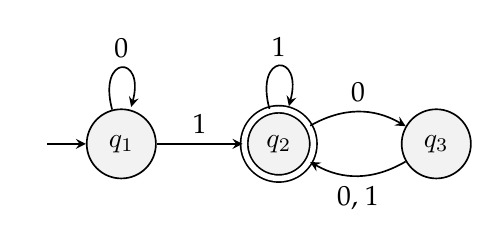
\begin{tikzpicture}
        \node[state, initial] (q1) {$q_1$};
        \node[state, accepting, right of=q1] (q2) {$q_2$};
        \node[state, right of=q2] (q3) {$q_3$};
        \draw	(q1) edge[loop above] node{0} (q1)
                (q1) edge[above] node{1} (q2)
                (q2) edge[loop above] node{1} (q2)
                (q2) edge[bend left, above] node{0} (q3)
                (q3) edge[bend left, below] node{0, 1} (q2);
    \end{tikzpicture}
    
    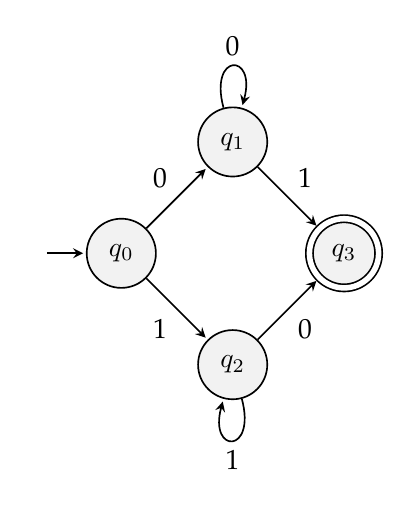
\begin{tikzpicture}[shorten >=1pt,node distance=2cm,on grid,auto] 
        \node[state,initial] (q_0)   {$q_0$}; 
        \node[state] (q_1) [above right=of q_0] {$q_1$}; 
        \node[state] (q_2) [below right=of q_0] {$q_2$}; 
        \node[state,accepting](q_3) [below right=of q_1] {$q_3$};
        \path[->] 
            (q_0) edge              node        {0} (q_1)
                  edge              node [swap] {1} (q_2)
            (q_1) edge              node        {1} (q_3)
                  edge [loop above] node        {0} ()
            (q_2) edge              node [swap] {0} (q_3) 
                  edge [loop below] node        {1} ();
    \end{tikzpicture}
    
    %--- Page 2 --------------------------------------------------------------------
    \newpage    

	\begin{minipage}{0.7\textwidth}
        $Q = \left\{ \; q_1, q_2, q_3 \; \right\} $ \quad
        $\Sigma = \left\{ \; 0, 1 \; \right\} $ \quad
        $S = \left\{ \; q_1, q_2 \; \right\} $ \quad
        $F = \left\{ \; q_3 \; \right\} $
	\end{minipage}
	\begin{minipage}{0.3\textwidth}
        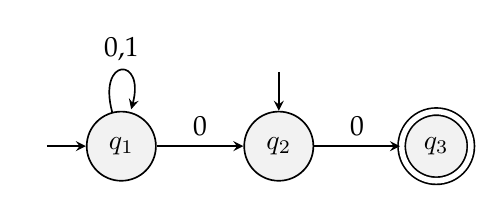
\begin{tikzpicture}
            \node[state, initial] (q1) {$q_1$};
            \node[state, initial above, right of=q1] (q2) {$q_2$};
            \node[state, accepting, right of=q2] (q3) {$q_3$};
            \draw	(q1) edge[loop above] node{0,1} (q1)
                    (q1) edge[above] node{0} (q2)
                    (q2) edge[above] node{0} (q3);
        \end{tikzpicture}
	\end{minipage}
    \vspace{-0.4cm}
    \begin{flalign*}
	    Q' &= \mathcal{P}\left(Q\right) = 2^{\vert Q \vert} = \left\{ \; \emptyset, \left\{ q_1 \right\}, \left\{ q_2 \right\}, \left\{ q_3 \right\}, \left\{ q_1, q_2 \right\}, \left\{ q_1, q_3 \right\}, \left\{ q_2, q_3 \right\}, \left\{ q_1, q_2, q_3 \right\} \; \right\} & \\
	    s' &= E\left( \left\{ S \right\} \right) = \left\{ \; q_1, q_2 \; \right\} & \\
	    F' &= \left\{ R \subseteq Q' \mid R \cap F \neq \emptyset \right\} = \left\{ \; \left\{ q_3 \right\}, \left\{ q_1, q_3 \right\}, \left\{ q_2, q_3 \right\}, \left\{ q_1, q_2, q_3 \right\} \; \right\} & \\
	\end{flalign*}
    \vspace{-1.6cm}
    \begin{tabular}{l|ccc|ll|ccc|ll|ccc|l}
        % 3-Tabelle: qi
        % -> 0
            \multicolumn{1}{c}{DFA:} & $q_1$    & $\xrightarrow{0}$ & \multicolumn{1}{c}{} & & 
            \multicolumn{1}{c}{}     & $q_2$    & $\xrightarrow{0}$ & \multicolumn{1}{c}{} & & 
            \multicolumn{1}{c}{}     & $q_3$    & $\xrightarrow{0}$ & \multicolumn{1}{c}{} &
        \\  
            \cline{2-4} \cline{7-9} \cline{12-14}
            NFA:                     & $q_1$   & $\xrightarrow{0}$  & $q_1,q_2$   & $\cup = q_1,q_2 $    &
                                     & $q_2$   & $\xrightarrow{0}$  & $q_3$       & $\cup = q_3$         &
                                     & $q_3$   & $\xrightarrow{0}$  & $\emptyset$ & $\cup = \emptyset$
        \\
            \cline{2-4} \cline{7-9} \cline{12-14}
            \multicolumn{1}{c}{} & & & \multicolumn{1}{c}{} & &
            \multicolumn{1}{c}{} & & & \multicolumn{1}{c}{} & &
            \multicolumn{1}{c}{} & & & \multicolumn{1}{c}{} &
        \\
        % -> 1
            \multicolumn{1}{c}{DFA:} & $q_1$    & $\xrightarrow{1}$ & \multicolumn{1}{c}{} & & 
            \multicolumn{1}{c}{}     & $q_2$    & $\xrightarrow{1}$ & \multicolumn{1}{c}{} & & 
            \multicolumn{1}{c}{}     & $q_3$    & $\xrightarrow{1}$ & \multicolumn{1}{c}{} &
        \\  
            \cline{2-4} \cline{7-9} \cline{12-14}
            NFA:                     & $q_1$    & $\xrightarrow{1}$ & $q1$        & $\cup = q_1$          &
                                     & $q_2$    & $\xrightarrow{1}$ & $\emptyset$ & $\cup = \emptyset$  &
                                     & $q_3$    & $\xrightarrow{1}$ & $\emptyset$ & $\cup = \emptyset$
        \\
            \cline{2-4} \cline{7-9} \cline{12-14}
            \multicolumn{1}{c}{} & & & \multicolumn{1}{c}{} & &
            \multicolumn{1}{c}{} & & & \multicolumn{1}{c}{} & &
            \multicolumn{1}{c}{} & & & \multicolumn{1}{c}{} &
        \\
        % 3-Tabelle: qi,qj
        % -> 0
            \multicolumn{1}{c}{DFA:} & $q_1q_2$ & $\xrightarrow{0}$ & \multicolumn{1}{c}{} & & 
            \multicolumn{1}{c}{}     & $q_1q_3$ & $\xrightarrow{0}$ & \multicolumn{1}{c}{} & & 
            \multicolumn{1}{c}{}     & $q_2q_3$ & $\xrightarrow{0}$ & \multicolumn{1}{c}{} &
        \\  
            \cline{2-4} \cline{7-9} \cline{12-14}
            \multirow{2}{*}{NFA:}    & $q_1$    & $\xrightarrow{0}$ & $q_1,q_2$   & \multirow{2}{*}{$\cup = q_1,q_2,q_3$} &
            \multirow{2}{*}{}        & $q_1$    & $\xrightarrow{0}$ & $q_1,q_2$   & \multirow{2}{*}{$\cup = q_1,q_2$} &
            \multirow{2}{*}{}        & $q_2$    & $\xrightarrow{0}$ & $q_3$       & \multirow{2}{*}{$\cup = q_3$}
        \\
                                     & $q_2$    & $\xrightarrow{0}$ & $q_3$       & &
                                     & $q_3$    & $\xrightarrow{0}$ & $\emptyset$ & &
                                     & $q_3$    & $\xrightarrow{0}$ & $\emptyset$ &
        \\
            \cline{2-4} \cline{7-9} \cline{12-14}
            \multicolumn{1}{c}{} & & & \multicolumn{1}{c}{} & &
            \multicolumn{1}{c}{} & & & \multicolumn{1}{c}{} & &
            \multicolumn{1}{c}{} & & & \multicolumn{1}{c}{} &
        \\
        % 3-Tabelle
        % -> 1
            \multicolumn{1}{c}{DFA:} & $q_1q_2$ & $\xrightarrow{1}$ & \multicolumn{1}{c}{} & & 
            \multicolumn{1}{c}{}     & $q_1q_3$ & $\xrightarrow{1}$ & \multicolumn{1}{c}{} & & 
            \multicolumn{1}{c}{}     & $q_2q_3$ & $\xrightarrow{1}$ & \multicolumn{1}{c}{} &
        \\  
            \cline{2-4} \cline{7-9} \cline{12-14}
            \multirow{2}{*}{NFA:}    & $q_1$    & $\xrightarrow{1}$ & $q_1$       & \multirow{2}{*}{$\cup = q_1$} &
            \multirow{2}{*}{}        & $q_1$    & $\xrightarrow{1}$ & $q_1$       & \multirow{2}{*}{$\cup = q_1$} &
            \multirow{2}{*}{}        & $q_2$    & $\xrightarrow{1}$ & $\emptyset$ & \multirow{2}{*}{$\cup = \emptyset$}
        \\
                                     & $q_2$    & $\xrightarrow{1}$ & $\emptyset$ & &
                                     & $q_3$    & $\xrightarrow{1}$ & $\emptyset$ & &
                                     & $q_3$    & $\xrightarrow{1}$ & $\emptyset$ &
        \\
            \cline{2-4} \cline{7-9} \cline{12-14}
            \multicolumn{1}{c}{} & & & \multicolumn{1}{c}{} & &
            \multicolumn{1}{c}{} & & & \multicolumn{1}{c}{} & &
            \multicolumn{1}{c}{} & & & \multicolumn{1}{c}{} &
        \\
        % 3-Tabelle: qi,qj,qk
        % -> 0, 1
            \multicolumn{1}{c}{DFA:} & $q_1q_2q_3$ & $\xrightarrow{0}$ & \multicolumn{1}{c}{} & & 
            \multicolumn{1}{c}{}     & $q_1q_2q_3$ & $\xrightarrow{1}$ & \multicolumn{1}{c}{} & & 
            \multicolumn{4}{c}{}     &
        \\  
            \cline{2-4} \cline{7-9}
            \multirow{3}{*}{NFA:}    & $q_1$    & $\xrightarrow{0}$ & $q_1,q_2$   & \multirow{3}{*}{$\cup = q_1,q_2,q_3$} &
            \multirow{3}{*}{}        & $q_1$    & $\xrightarrow{1}$ & $q_1$       & \multirow{3}{*}{$\cup = q_1$} &
            \multicolumn{4}{c}{}     &
        \\
                                     & $q_2$    & $\xrightarrow{0}$ & $q_3$       & &
                                     & $q_3$    & $\xrightarrow{1}$ & $\emptyset$ & &
            \multicolumn{4}{c}{}     &
        \\
                                     & $q_2$    & $\xrightarrow{0}$ & $\emptyset$ & &
                                     & $q_3$    & $\xrightarrow{1}$ & $\emptyset$ & &
            \multicolumn{4}{c}{}     &
        \\
            \cline{2-4} \cline{7-9}
            \multicolumn{1}{c}{} & & & \multicolumn{1}{c}{} & &
            \multicolumn{1}{c}{} & & & \multicolumn{1}{c}{} & &
            \multicolumn{1}{c}{} & & & \multicolumn{1}{c}{} &
        \\
            
    \end{tabular}
    
	\begin{minipage}{0.6\textwidth}
        
        \begin{tabular}{l|ccc|l}
            % 3-Tabelle: qi
            % -> 0
                \multicolumn{1}{c}{DFA:} & $q_xq_yq_z$ & $\xrightarrow{\omega_i}$ & \multicolumn{1}{c}{} & 
            \\  
                \cline{2-4}
                \multirow{3}{*}{NFA:}    & $q_x$ & $\xrightarrow{\omega_i}$ & $q_x$ & \multirow{3}{*}{$\cup = q_x,q_z$} 
            \\
                                         & $q_y$ & $\xrightarrow{\omega_i}$ & $q_z$ &
            \\
                                         & $q_z$ & $\xrightarrow{\omega_i}$ & $\emptyset$ &
            \\
                \cline{2-4}
                \multicolumn{1}{c}{} & & & \multicolumn{1}{c}{} &
            \\
        \end{tabular} \\
        \begin{tabular}{c|cc}
            $ \delta' $                          & 0                                 & 1                         \\
            \hline
            $ \emptyset $                       & $\emptyset$                       & $\emptyset$               \\
            $ \left\{ q_1 \right\} $            & $\left\{ q_1, q_2 \right\}$       & $\left\{ q_1 \right\}$    \\
            $ \left\{ q_2 \right\} $            & $ \left\{ q_3 \right\}$           & $\emptyset$               \\
            $ \left\{ q_3 \right\} $            & $\emptyset$                       & $\emptyset$               \\
            $ \left\{ q_1, q_2 \right\} $       & $\left\{ q_1, q_2, q_3 \right\}$  & $\left\{ q_1 \right\}$    \\
            $ \left\{ q_1, q_3 \right\} $       & $\left\{ q_1, q_2 \right\}$       & $\left\{ q_1 \right\}$    \\
            $ \left\{ q_2, q_3 \right\} $       & $\left\{ q_3 \right\}$            & $\emptyset$               \\
            $ \left\{ q_1, q_2, q_3 \right\} $  & $q_2$ & $q_2$
        \end{tabular}
	\end{minipage}
	\begin{minipage}{0.4\textwidth} 
        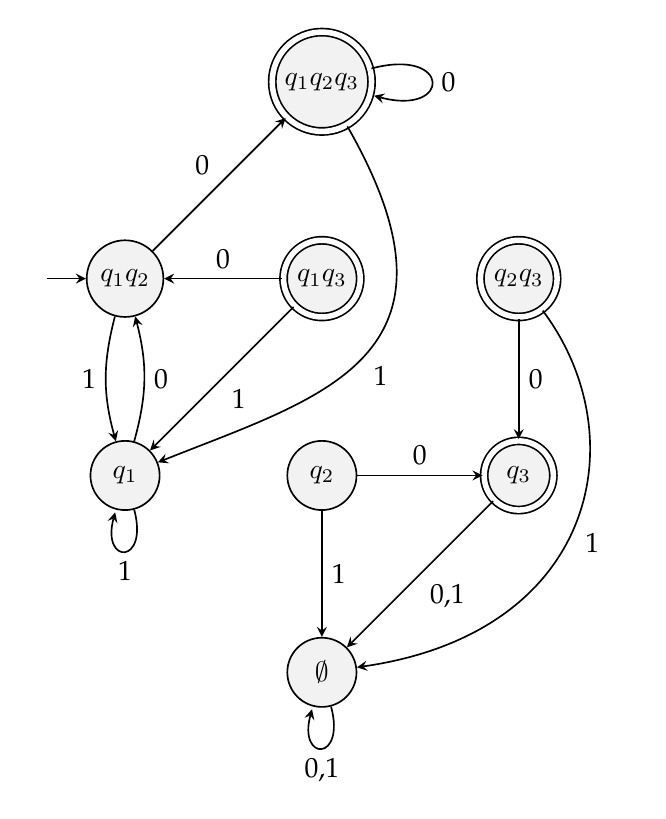
\begin{tikzpicture}[node distance=2.5cm]
            % erste zeile
            \node[state]                            (nul)       {$\emptyset$};
            % zweite zeile
            \node[state, above of=nul]              (q2)        {$q_2$};
            \node[state, left of=q2]                (q1)        {$q_1$};
            \node[state, accepting, right of=q2]    (q3)        {$q_3$};
            % dritte zeile
            \node[state, accepting, above of=q2]    (q1q3)      {$q_1q_3$};
            \node[state, initial, left of=q1q3]     (q1q2)      {$q_1q_2$};
            \node[state, accepting, right of=q1q3]  (q2q3)      {$q_2q_3$};
            % vierte zeile
            \node[state, accepting, above of=q1q3]  (q1q2q3)    {$q_1q_2q_3$};
    
            \draw[->,>=stealth,auto,semithick]
                    % erste zeile
                    (nul)   edge[loop below]        node{0,1}   ()
                    % zweite zeile
                    (q1)    edge[loop below]        node{1}     ()
                    (q1)    edge[bend angle=15,
                                 bend right,right]  node{0}     (q1q2)
                    (q2)    edge                    node{0}     (q3)
                    (q2)    edge                    node{1}     (nul)
                    (q3)    edge                    node{0,1}   (nul)
                    % dritte zeile
                    (q1q2)  edge[bend angle=15,
                                 bend right,left]   node{1}     (q1)
                    (q1q2)  edge                    node{0}     (q1q2q3)
                    (q1q3)  edge[above]             node{0}     (q1q2)
                    (q1q3)  edge                    node{1}     (q1)
                    (q2q3)  edge                    node{0}     (q3)
                    % vierte zeile
                    (q1q2q3) edge[loop right]       node{0}     ()
            ;
            \draw[->,>=stealth,auto,semithick]
                    %(q2q3)  to [out = -50, in = 0]
                    %          node{0}     (nul)
                    (q2q3)  .. controls (4,3)
                               and      (3.5,0.5) .. node{1}    (nul);
            \draw[->,>=stealth,auto,semithick]
                    (q1q2q3) .. controls (2,4)
                                and      (0,3.5) .. node{1}     (q1);
            %\draw (q1q2q3) .. controls (0,4) and (4,0) .. (q1);
            %\draw[step=1cm,gray,very thin] (-2,0) grid (2,4);
        \end{tikzpicture}
	\end{minipage}

    %--- Page 3 --------------------------------------------------------------------
    \newpage

	\begin{minipage}{0.7\textwidth}
        $Q = \left\{ \; q_1, q_2, q_3 \; \right\} $ \quad
        $\Sigma = \left\{ \; 0, 1 \; \right\} $ \quad
        $S = \left\{ \; q_1, q_2 \; \right\} $ \quad
        $F = \left\{ \; q_3 \; \right\} $
	\end{minipage}
	\begin{minipage}{0.3\textwidth}
        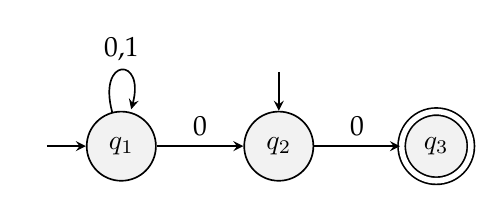
\begin{tikzpicture}
            \node[state, initial] (q1) {$q_1$};
            \node[state, initial above, right of=q1] (q2) {$q_2$};
            \node[state, accepting, right of=q2] (q3) {$q_3$};
            \draw	(q1) edge[loop above] node{0,1} (q1)
                    (q1) edge[above] node{0} (q2)
                    (q2) edge[above] node{0} (q3);
        \end{tikzpicture}
	\end{minipage}

	\begin{minipage}[t]{0.5\textwidth}
        \def\h{0.5cm}
        \def\w{2cm}
        \begin{tabular}[t]{c|cc}
            $ \delta' $                         & a                             & b                             \\
            \hline
            $ \emptyset $                       & \parbox[b][\h][c]{\w}{\quad}  & \parbox[b][\h][c]{\w}{\quad}  \\
            $ \left\{ q_1 \right\} $            & \parbox[b][\h][c]{\w}{\quad}  & \parbox[b][\h][c]{\w}{\quad}  \\
            $ \left\{ q_2 \right\} $            & \parbox[b][\h][c]{\w}{\quad}  & \parbox[b][\h][c]{\w}{\quad}  \\
            $ \left\{ q_3 \right\} $            & \parbox[b][\h][c]{\w}{\quad}  & \parbox[b][\h][c]{\w}{\quad}  \\
            $ \left\{ q_1, q_2 \right\} $       & \parbox[b][\h][c]{\w}{\quad}  & \parbox[b][\h][c]{\w}{\quad}  \\
            $ \left\{ q_1, q_3 \right\} $       & \parbox[b][\h][c]{\w}{\quad}  & \parbox[b][\h][c]{\w}{\quad}  \\
            $ \left\{ q_2, q_3 \right\} $       & \parbox[b][\h][c]{\w}{\quad}  & \parbox[b][\h][c]{\w}{\quad}  \\
            $ \left\{ q_1, q_2, q_3 \right\} $  & \parbox[b][\h][c]{\w}{\quad}  & \parbox[b][\h][c]{\w}{\quad}
       \end{tabular}
	\end{minipage}
	\begin{minipage}[t]{0.5\textwidth}
        \def\h{0.5cm}
        \def\w{2cm}
        \begin{tabular}[t]{c|cc}
            $ \delta' $                          & a                                 & b                         \\
            \hline
            $ \emptyset $                       & \parbox[b][\h][c]{\w}{\quad}  & \parbox[b][\h][c]{\w}{\quad}  \\
            $ \left\{ q_1 \right\} $            & \parbox[b][\h][c]{\w}{\quad}  & \parbox[b][\h][c]{\w}{\quad}  \\
            $ \left\{ q_2 \right\} $            & \parbox[b][\h][c]{\w}{\quad}  & \parbox[b][\h][c]{\w}{\quad}  \\
            $ \left\{ q_3 \right\} $            & \parbox[b][\h][c]{\w}{\quad}  & \parbox[b][\h][c]{\w}{\quad}  \\
            $ \left\{ q_1, q_2 \right\} $       & \parbox[b][\h][c]{\w}{\quad}  & \parbox[b][\h][c]{\w}{\quad}  \\
            $ \left\{ q_1, q_3 \right\} $       & \parbox[b][\h][c]{\w}{\quad}  & \parbox[b][\h][c]{\w}{\quad}  \\
            $ \left\{ q_2, q_3 \right\} $       & \parbox[b][\h][c]{\w}{\quad}  & \parbox[b][\h][c]{\w}{\quad}  \\
            $ \left\{ q_1, q_2, q_3 \right\} $  & \parbox[b][\h][c]{\w}{\quad}  & \parbox[b][\h][c]{\w}{\quad}  
        \end{tabular}
	\end{minipage}

    \quad

    \quad

    \quad

	\begin{minipage}{0.7\textwidth}
        $Q = \left\{ \; q_1, q_2, q_3 \; \right\} $ \quad
        $\Sigma = \left\{ \; a, b \; \right\} $ \quad
        $S = \left\{ \; q_1 \; \right\} $ \quad
        $F = \left\{ \; q_1 \; \right\} $
	\end{minipage}
	\begin{minipage}{0.3\textwidth}
        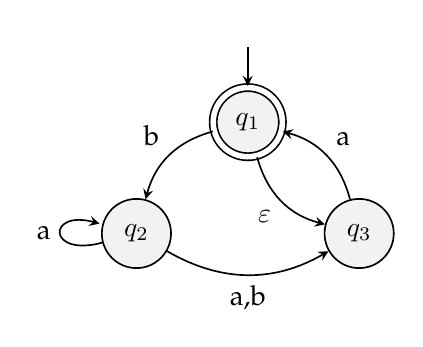
\begin{tikzpicture}
            \node[state, accepting, initial above] (q1) {$q_1$};
            \node[state, below left of=q1] (q2) {$q_2$};
            \node[state, below right of=q1] (q3) {$q_3$};
            \draw   (q1) edge[bend right, below left]   node{$\varepsilon$} (q3)
                    (q1) edge[bend right, above left]   node{b}             (q2)
                    (q2) edge[bend right, below]        node{a,b}           (q3)
                    (q2) edge[loop left]                node{a}             (q2)
                    (q3) edge[bend right, above right]  node{a}             (q1);
        \end{tikzpicture}
	\end{minipage}

	\begin{minipage}[t]{0.5\textwidth}
        \def\h{0.5cm}
        \def\w{2cm}
        \begin{tabular}[t]{c|cc}
            $ \delta' $                         & a                             & b                             \\
            \hline
            $ \emptyset $                       & \parbox[b][\h][c]{\w}{\quad}  & \parbox[b][\h][c]{\w}{\quad}  \\
            $ \left\{ q_1 \right\} $            & \parbox[b][\h][c]{\w}{\quad}  & \parbox[b][\h][c]{\w}{\quad}  \\
            $ \left\{ q_2 \right\} $            & \parbox[b][\h][c]{\w}{\quad}  & \parbox[b][\h][c]{\w}{\quad}  \\
            $ \left\{ q_3 \right\} $            & \parbox[b][\h][c]{\w}{\quad}  & \parbox[b][\h][c]{\w}{\quad}  \\
            $ \left\{ q_1, q_2 \right\} $       & \parbox[b][\h][c]{\w}{\quad}  & \parbox[b][\h][c]{\w}{\quad}  \\
            $ \left\{ q_1, q_3 \right\} $       & \parbox[b][\h][c]{\w}{\quad}  & \parbox[b][\h][c]{\w}{\quad}  \\
            $ \left\{ q_2, q_3 \right\} $       & \parbox[b][\h][c]{\w}{\quad}  & \parbox[b][\h][c]{\w}{\quad}  \\
            $ \left\{ q_1, q_2, q_3 \right\} $  & \parbox[b][\h][c]{\w}{\quad}  & \parbox[b][\h][c]{\w}{\quad}
       \end{tabular}
	\end{minipage}
	\begin{minipage}[t]{0.5\textwidth}
        \def\h{0.5cm}
        \def\w{2cm}
        \begin{tabular}[t]{c|cc}
            $ \delta' $                          & a                                 & b                         \\
            \hline
            $ \emptyset $                       & \parbox[b][\h][c]{\w}{\quad}  & \parbox[b][\h][c]{\w}{\quad}  \\
            $ \left\{ q_1 \right\} $            & \parbox[b][\h][c]{\w}{\quad}  & \parbox[b][\h][c]{\w}{\quad}  \\
            $ \left\{ q_2 \right\} $            & \parbox[b][\h][c]{\w}{\quad}  & \parbox[b][\h][c]{\w}{\quad}  \\
            $ \left\{ q_3 \right\} $            & \parbox[b][\h][c]{\w}{\quad}  & \parbox[b][\h][c]{\w}{\quad}  \\
            $ \left\{ q_1, q_2 \right\} $       & \parbox[b][\h][c]{\w}{\quad}  & \parbox[b][\h][c]{\w}{\quad}  \\
            $ \left\{ q_1, q_3 \right\} $       & \parbox[b][\h][c]{\w}{\quad}  & \parbox[b][\h][c]{\w}{\quad}  \\
            $ \left\{ q_2, q_3 \right\} $       & \parbox[b][\h][c]{\w}{\quad}  & \parbox[b][\h][c]{\w}{\quad}  \\
            $ \left\{ q_1, q_2, q_3 \right\} $  & \parbox[b][\h][c]{\w}{\quad}  & \parbox[b][\h][c]{\w}{\quad}  
        \end{tabular}
	\end{minipage}

    %--- Page 4 --------------------------------------------------------------------
    \newpage
    
	\begin{minipage}{0.7\textwidth}
        $Q = \left\{ \; q_1, q_2, q_3 \; \right\} $ \quad
        $\Sigma = \left\{ \; a, b \; \right\} $ \quad
        $S = \left\{ \; q_1 \; \right\} $ \quad
        $F = \left\{ \; q_1 \; \right\} $
	\end{minipage}
	\begin{minipage}{0.3\textwidth}
        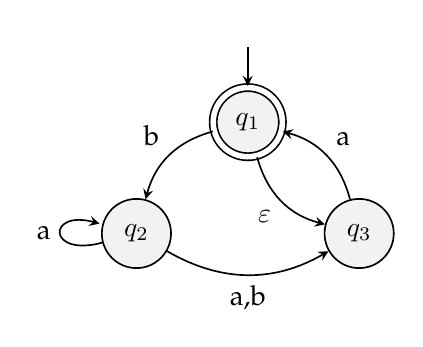
\begin{tikzpicture}
            \node[state, accepting, initial above] (q1) {$q_1$};
            \node[state, below left of=q1] (q2) {$q_2$};
            \node[state, below right of=q1] (q3) {$q_3$};
            \draw   (q1) edge[bend right, below left]   node{$\varepsilon$} (q3)
                    (q1) edge[bend right, above left]   node{b}             (q2)
                    (q2) edge[bend right, below]        node{a,b}           (q3)
                    (q2) edge[loop left]                node{a}             (q2)
                    (q3) edge[bend right, above right]  node{a}             (q1);
        \end{tikzpicture}
	\end{minipage}
    \vspace{-0.4cm}
    \begin{flalign*}
	    Q' &= \mathcal{P}\left(Q\right) = 2^{\vert Q \vert} = \left\{ \; \emptyset, \left\{ q_1 \right\}, \left\{ q_2 \right\}, \left\{ q_3 \right\}, \left\{ q_1, q_2 \right\}, \left\{ q_1, q_3 \right\}, \left\{ q_2, q_3 \right\}, \left\{ q_1, q_2, q_3 \right\} \; \right\} & \\
	    s' &= E\left( \left\{ S \right\} \right) = \left\{ \; q_1, q_3 \; \right\} & \\
	    F' &= \left\{ R \subseteq Q' \mid R \cap F \neq \emptyset \right\} = \left\{ \; \left\{ \uline{q_1} \right\}, \left\{ \uline{q_1}, q_2 \right\}, \left\{ \uline{q_1}, q_3 \right\}, \left\{ \uline{q_1}, q_2, q_3 \right\} \; \right\} & \\
	\end{flalign*}
   % \vspace{-1.6cm}

	\begin{minipage}[t]{0.5\textwidth}
        \begin{tabular}[t]{c|cc}
            $ \delta' $                         & a                                 & b                             \\
            \hline
            $ \emptyset $                       & $\emptyset$                       & $\emptyset$                   \\
            $ \left\{ q_1 \right\} $            & $\emptyset$                       & $\left\{ q_2 \right\}$        \\
            $ \left\{ q_2 \right\} $            & $\left\{ q_2, q_3 \right\}$       & $\left\{ q_3 \right\}$        \\
            $ \left\{ q_3 \right\} $            & $\left\{ q_1, q_3 \right\}$       & $\emptyset$                   \\
            $ \left\{ q_1, q_2 \right\} $       & $\left\{ q_1, q_3 \right\}$       & $\left\{ q_2, q_3 \right\}$   \\
            $ \left\{ q_1, q_3 \right\} $       & $\left\{ q_1, q_3 \right\}$       & $\left\{ q_2 \right\}$        \\
            $ \left\{ q_2, q_3 \right\} $       & $\left\{ q_1, q_2, q_3 \right\}$  & $\left\{ q_3 \right\}$        \\
            $ \left\{ q_1, q_2, q_3 \right\} $  & $\left\{ q_1, q_2, q_3 \right\}$  & $\left\{ q_2, q_3 \right\}$
        \end{tabular}
	\end{minipage}
	\begin{minipage}[t]{0.5\textwidth}
        \begin{tabular}[t]{c|cc}
            $ \delta' $                         & a                                 & b                             \\
            \hline
            $ \left\{ q_1, q_3 \right\} $       & $\left\{ q_1, q_3 \right\}$       & $\left\{ q_2 \right\}$        \\
            $ \left\{ q_2 \right\} $            & $\left\{ q_2, q_3 \right\}$       & $\left\{ q_3 \right\}$        \\
            $ \left\{ q_2, q_3 \right\} $       & $\left\{ q_1, q_2, q_3 \right\}$  & $\left\{ q_3 \right\}$        \\
            $ \left\{ q_1, q_2, q_3 \right\} $  & $\left\{ q_1, q_2, q_3 \right\}$  & $\left\{ q_2, q_3 \right\}$   \\
            $ \left\{ q_3 \right\} $            & $\left\{ q_1, q_3 \right\}$       & $\emptyset$                   \\
            $ \emptyset $                       & $\emptyset$                       & $\emptyset$
        \end{tabular}
	\end{minipage}

    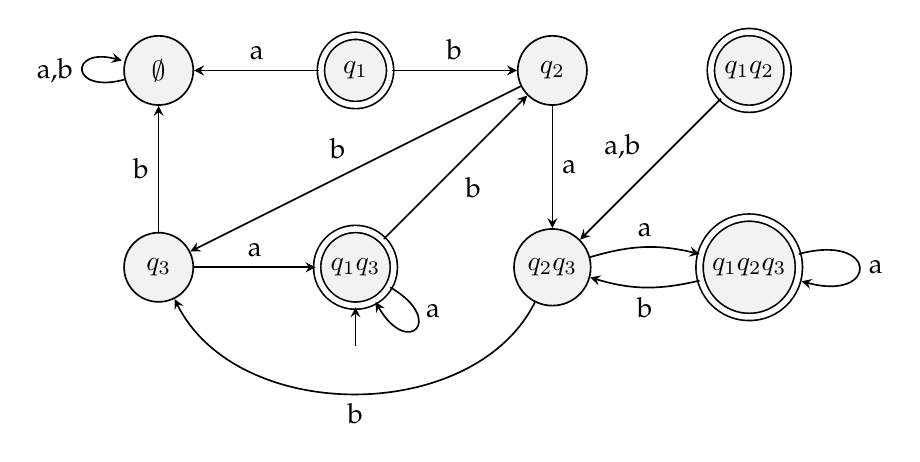
\begin{tikzpicture}[node distance=2.5cm]
        % erste zeile
        \node[state]                            (nul)       {$\emptyset$};
        \node[state, accepting, right of=nul]   (q1)        {$q_1$};
        \node[state, right of=q1]               (q2)        {$q_2$};
        \node[state, accepting, right of=q2]    (q1q2)      {$q_1q_2$};
        % zweite zeile
        \node[state, below of=nul]              (q3)        {$q_3$};
        \node[state, initial below, accepting, right of=q3]    (q1q3)      {$q_1q_3$};
        \node[state, right of=q1q3]             (q2q3)      {$q_2q_3$};
        \node[state, accepting, right of=q2q3]  (q1q2q3)    {$q_1q_2q_3$};

        \draw[->,>=stealth,auto,semithick]
                % erste zeile
                (nul)   edge[loop left]             node{a,b}   ()
                (q1)    edge[above]                 node{a}     (nul)
                (q1)    edge[]                      node{b}     (q2)
                (q2)    edge[]                      node{a}     (q2q3)
                (q2)    edge[above left]            node{b}     (q3)
                (q1q2)  edge[above left]            node{a,b}   (q2q3)
                % zweite zeile
                (q3)    edge[]                      node{b}     (nul)
                (q3)    edge[]                      node{a}     (q1q3)
                (q1q3)  edge[below right]           node{b}     (q2)
                (q1q3)  edge [out=330,in=300,
                              looseness=8,
                              above right]          node{a}     (q1q3)
                (q2q3)  edge[bend angle=15,
                             bend left]             node{a}     (q1q2q3)
                (q2q3)  .. controls (4,-4.5)
                               and      (1,-4.5) .. node{b}     (q3)
                (q1q2q3) edge[loop right]           node{a}     ()
                (q1q2q3) edge[bend angle=15,
                             bend left, below]      node{b}     (q2q3)
        ;
        %\draw (q1q2q3) .. controls (0,4) and (4,0) .. (q1);
        %\draw[step=1cm,gray,very thin] (-2,0) grid (2,4);
    \end{tikzpicture}

    %--- Page 5 --------------------------------------------------------------------
    \newpage
    
    \begin{flalign*}
        \Sigma        & = \left\{ \; a, b, \ldots, z \; \right\} & \\
        L_1           & = \left\{ \; \textrm{good}, \textrm{bad} \; \right\} \quad L_2 = \left\{ \; \textrm{dog}, \textrm{cat} \; \right\}& \\
        L_1 \cup L_2  & = \left\{ \; \textrm{good}, \textrm{bad}, \textrm{dog}, \textrm{cat} \; \right\} & \\
        L_1 \cdot L_2 & = \left\{ \; \textrm{gooddog}, \textrm{goodcat}, \textrm{baddog}, \textrm{badcat} \; \right\} & \\
        L_2^0         & = \left\{ \; \varepsilon \; \right\} & \\
        L_2^1         & = \left\{ \; \textrm{dog}, \textrm{cat} \; \right\} & \\
        L_2^2         & = \left\{ \; \textrm{dogdog}, \textrm{dogcat}, \textrm{catdog}, \textrm{catcat} \; \right\} & \\
        L_2^3         & = L_2 \cdot L_2 \cdot L_2 & \\
        & = \left\{ \; \textrm{dog}, \textrm{cat} \; \right\} \cdot \left\{ \; \textrm{dog}, \textrm{cat} \; \right\} \cdot \left\{ \; \textrm{dog}, \textrm{cat} \; \right\} & \\
        & = \left\{ \; \textrm{dogdogdog}, \textrm{dogdogcat}, \textrm{dogcatdog}, \textrm{dogcatcat},  \ldots \; \right\} & \\
        L_2^*         & = L_2^0 \cup L_2^1 \cup L_2^2 \cup \ldots & \\
        & = \left\{ \; \varepsilon,
        \textrm{dog}, \textrm{cat},
        \textrm{dogdog}, \textrm{dogcat}, \ldots \; \right\} & \\
    \end{flalign*} \\
    
    \textbf{Deterministic Finite Automaton (DFA):}\\
    Ein DFA ist ein 5-Tupel $(Q,\Sigma,\delta, s, F)$ wobei \\
    \hspace{-0.3cm}
    \begin{tabular}{lll}
        1) & $Q$                                             & endliche Menge von Zuständen \\
        2) & $\Sigma$                                        & Eingangsalphabet \\
        3) & $\delta: Q \times \Sigma \xrightarrow{\;\;} Q$: & einen nachfolgenden Zustand \\
           & $\delta\left(r_{i},\omega_i \right) = r_{i+1} $ & $r_i \in Q$\\
        4) & $s \in Q$                                       & Startzustand \\
        5) & $F \subseteq Q$                                 & Menge akzeptierender Zustände
    \end{tabular}

    \textbf{Nondeterministic Finite Automaton (NFA):}\\
    Ein NFA ist ein 5-Tupel $(Q,\Sigma,\delta, S, F)$ wobei \\
    \hspace{-0.3cm}
    \begin{tabular}{lll}
        1) & $Q$                                             & endliche Menge von Zuständen \\
        2) & $\Sigma$                                        & Eingangsalphabet \\
        3) & $\delta: Q \times \Sigma_\varepsilon \xrightarrow{\;\;} \mathcal{P}\left(Q\right)$: & mehrere nachfolgende Zustände \\
           &                                                 & Potenzmenge $\mathcal{P}\left(Q\right)$, $ \Sigma_\varepsilon = \Sigma \cup \left\{ \varepsilon \right\} $ \\
        4) & $S \subseteq Q$                                 & Menge von Startzuständen \\
        5) & $F \subseteq Q$                                 & Menge akzeptierender Zustände
    \end{tabular} \\
    Überführung in DFA $(Q',\Sigma,\delta', s', F')$\\
    \begin{tabular}{lll}
        1) & $Q'=2^{\vert Q \vert}$                          & \\
        2) & \multicolumn{2}{l}{$ E\left( R \right) = \left\{ r \in Q \mid r \text{ erreichbar von } R \text{ mit } 0 \text{ oder mehr } \varepsilon \text{-Transitionen} \right\} $} \\
        3) & $\bigcup\limits_{r \in R} E \left( \delta\left(r_{i},\omega_i \right) \right) $ & \\
        4) & $s' = E\left( \left\{ S \right\} \right) $                                 & \\
        5) & $F'= \left\{ R \subseteq Q' \mid R \cap F \neq \emptyset \right\}$                                 &
    \end{tabular}

    %--- Page 6 --------------------------------------------------------------------
    \newpage


\end{document}
